\documentclass[11pt]{article}

\usepackage[margin=0.85in]{geometry}
\usepackage[T1]{fontenc}
\usepackage[utf8]{inputenc}
\usepackage{lmodern}
\usepackage{microtype}
\usepackage{graphicx}
\usepackage{booktabs}
\usepackage{amsmath}
\usepackage{hyperref}
\usepackage{caption}
\usepackage{subcaption}
\usepackage{float}

\hypersetup{
  colorlinks=true,
  linkcolor=blue,
  citecolor=blue,
  urlcolor=blue
}

\newcommand{\outputroot}{/home/lachlan/ProjectsLFS/OrganoidAgent/analysis-outputs/yichao_future_expression}

\title{\textbf{Yichao Separate Training Results: Same-Time B2F and Scalar Future Prediction}}
\author{OrganoidAgent Yichao analysis}
\date{May 11, 2026}

\begin{document}
\maketitle

\begin{abstract}
This report covers only the separately trained Yichao models. Stage 1 trained a same-time brightfield-to-fluorescence image model ($B_t \rightarrow F_t$). Stage 2 trained a separate scalar future-expression model from earlier brightfield history and morphology features ($B_{0:k}, X_{0:k} \rightarrow s_{p>k}$). The same-time B2F model contains useful signal, with held-out image MAE 0.1077, expression AUROC 0.728, and fluorescence peak Pearson correlation 0.685. The separate scalar future model does not yet provide useful future prediction, with held-out expression AUROC 0.228 and future peak Pearson correlation 0.134. The practical conclusion from the separate training is that B2F should be kept as a representation-learning task, while scalar future prediction needs stronger temporal targets and a better longitudinal model.
\end{abstract}

\section{Scope}

This document intentionally excludes the joint model. It uses only the stage1 and stage2 artifacts:

\begin{itemize}
\item Stage 1 B2F model: \path{\outputroot/stage1_b2f}
\item Stage 1 B2F evaluation: \path{\outputroot/stage1_b2f_evaluation}
\item Stage 2 scalar future model: \path{\outputroot/stage2_future_expression}
\end{itemize}

\section{Dataset}

The projected complete/non-edge Yichao dataset was built at:

\begin{center}
\small
\path{\outputroot/future_expression.sqlite}
\end{center}

The B2F stage used 6,691 training crops, 1,601 validation crops, and 1,088 held-out test crops at 256$\times$256 pixels. The scalar future stage used 4,277 training prefix samples, 1,178 validation samples, and 633 held-out test samples. The scalar model used up to five prefix frames and explicit morphology/time features.

\section{Separate Model 1: Same-Time B2F}

The B2F model learns:
\begin{equation}
\hat{F}_t = G_\theta(B_t),
\end{equation}
where $B_t$ is a projected brightfield organoid crop and $F_t$ is the same-time projected fluorescence crop.

\begin{table}[H]
\centering
\caption{Held-out B2F test metrics from \texttt{stage1\_b2f\_evaluation/test\_metrics.json}.}
\begin{tabular}{lc}
\toprule
Metric & Value \\
\midrule
Test crops & 1,088 \\
Expression-labeled crops & 14 \\
Image MAE & 0.1077 \\
Image MSE & 0.0382 \\
Image PSNR & 14.18 dB \\
Expression AUROC & 0.728 \\
Average precision & 0.1097 \\
Peak Pearson correlation & 0.685 \\
Peak MAE & 0.746 \\
Best epoch & 3 \\
Device & CUDA \\
\bottomrule
\end{tabular}
\end{table}

\begin{figure}[H]
\centering
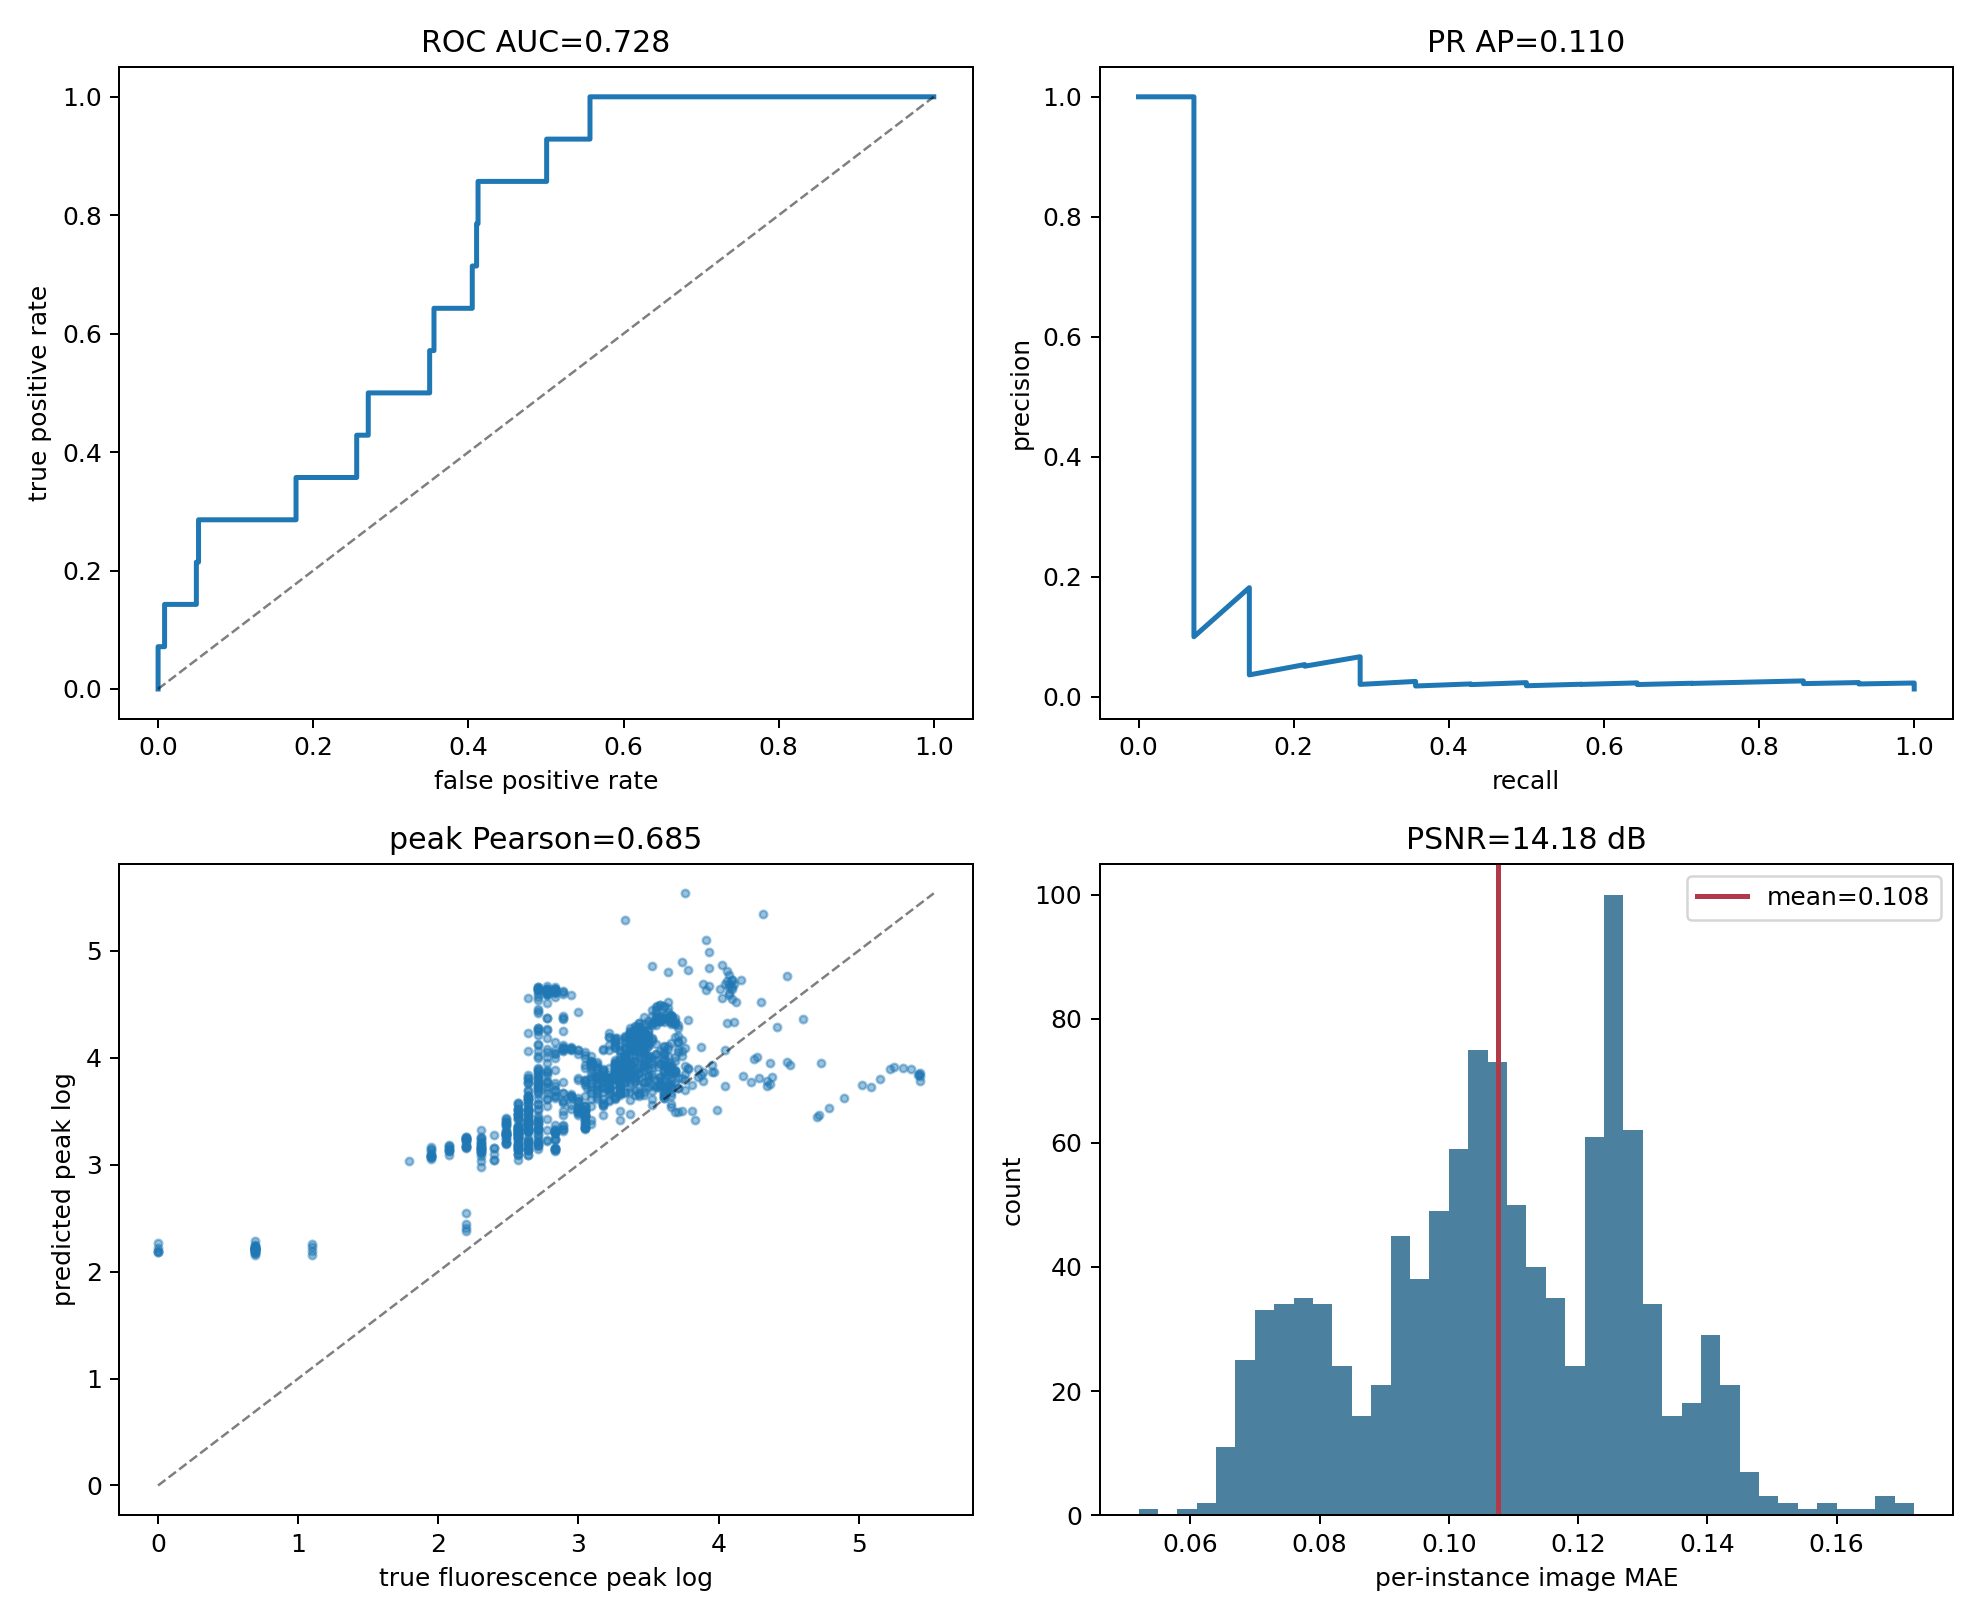
\includegraphics[width=\linewidth]{figures/fig1_b2f_performance_summary.png}
\caption{Same-time B2F performance summary from the separate B2F evaluation.}
\label{fig:b2f-summary}
\end{figure}

\begin{figure}[H]
\centering
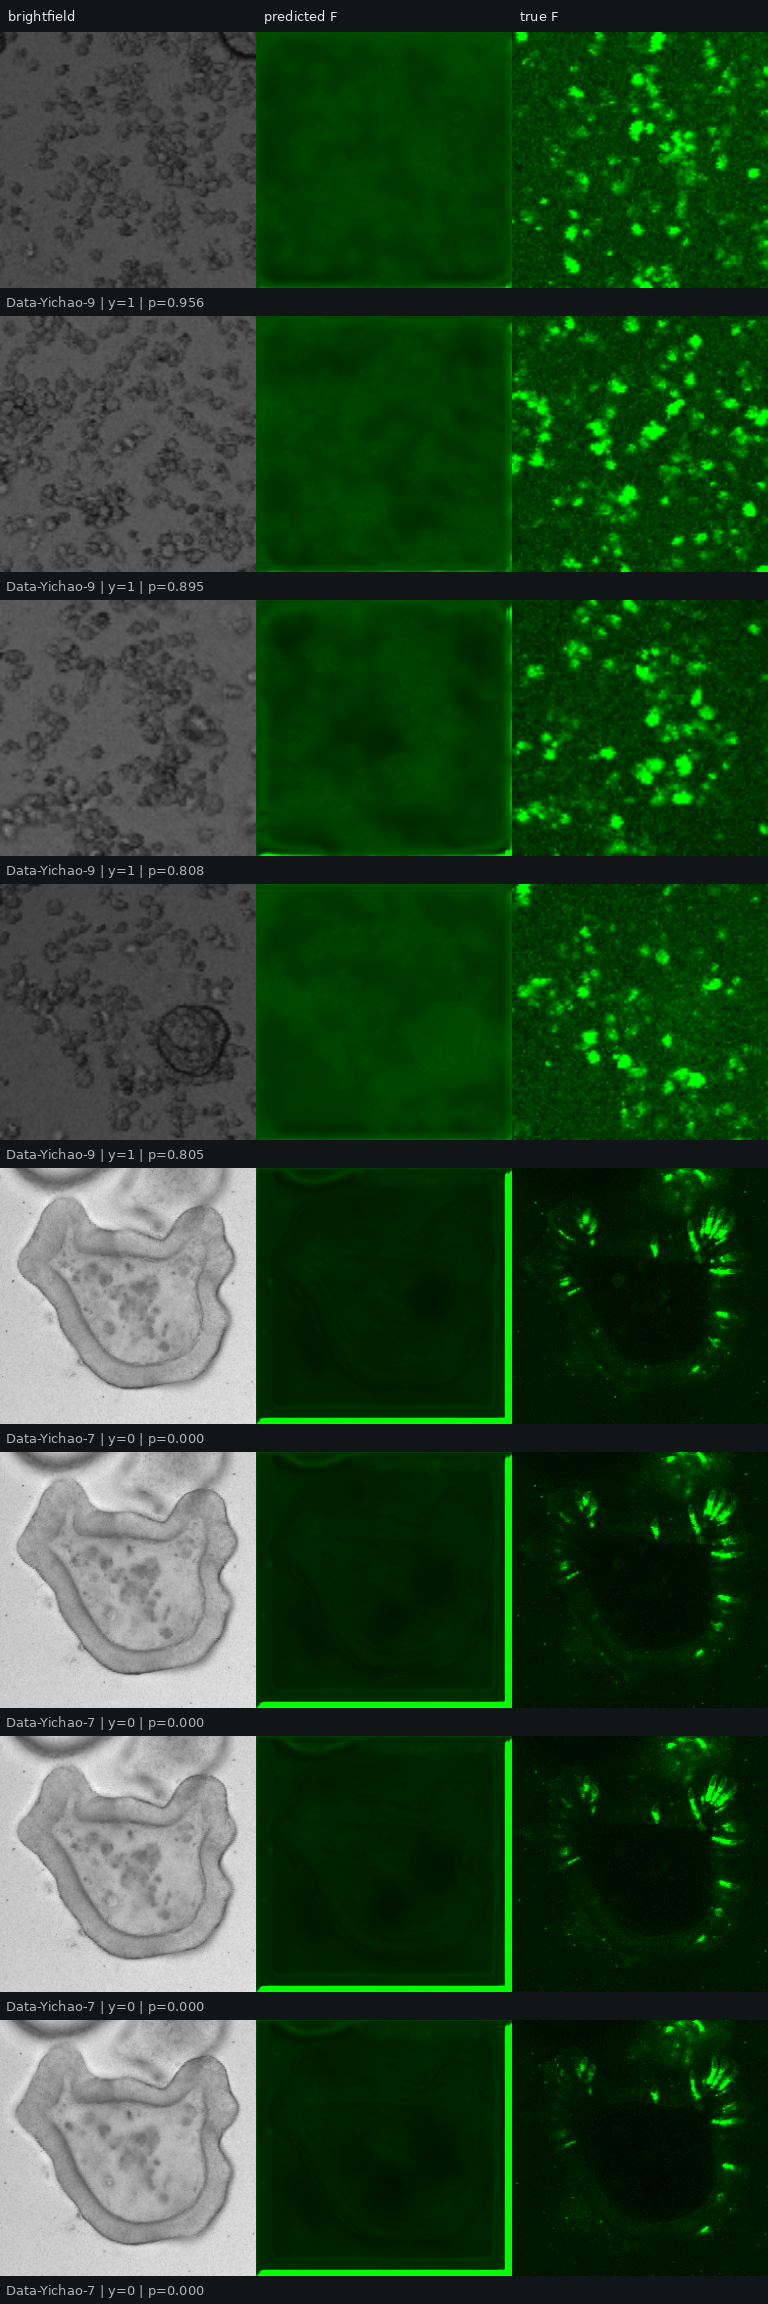
\includegraphics[height=0.82\textheight,keepaspectratio]{figures/fig2_b2f_predictions.png}
\caption{Held-out B2F examples. Columns show brightfield input, predicted fluorescence, and true fluorescence.}
\label{fig:b2f-examples}
\end{figure}

\section{Separate Feature Explanation}

The same-time B2F result suggests that projected brightfield morphology contains some information associated with same-time fluorescence. The explicit feature analysis is useful because it shows which interpretable morphology variables carry signal.

\begin{figure}[H]
\centering
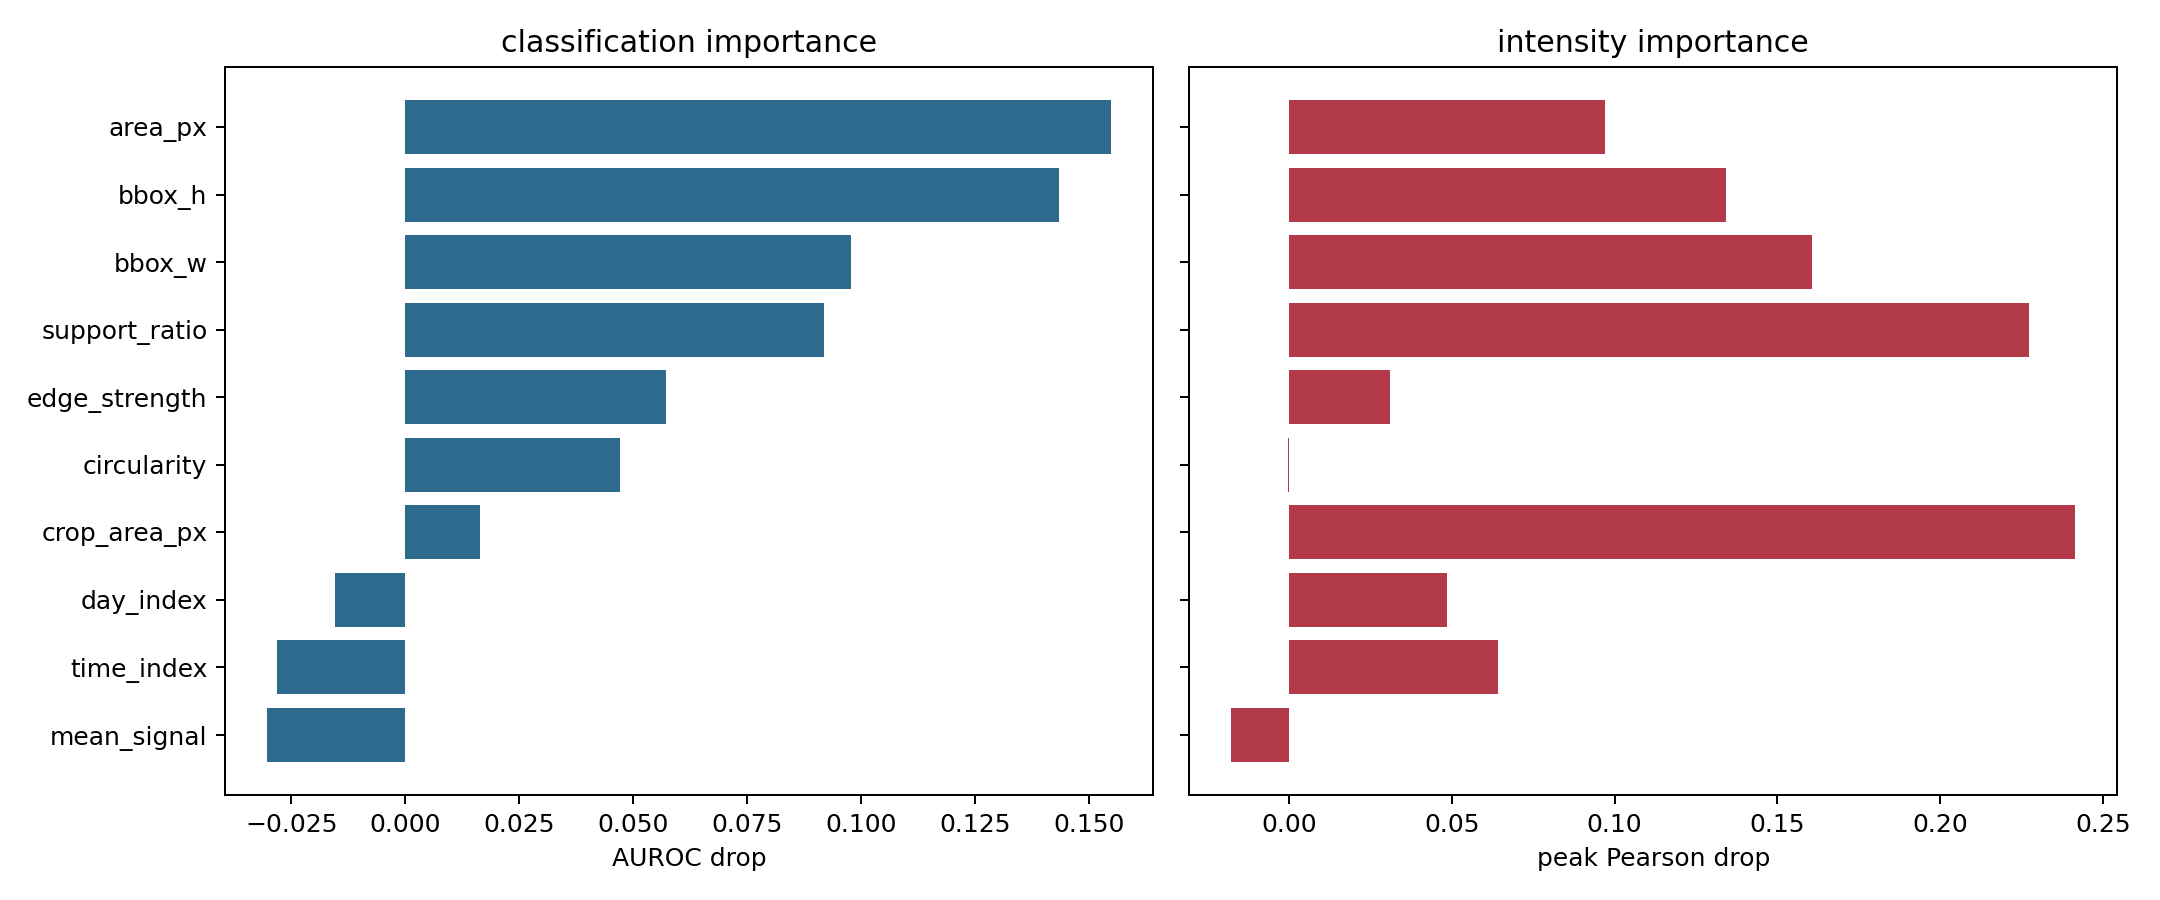
\includegraphics[width=0.92\linewidth]{figures/fig3_b2f_feature_importance.png}
\caption{Feature importance summary for same-time fluorescence distinction. Size, bounding-box geometry, support ratio, and edge features are the strongest explanatory variables.}
\label{fig:b2f-feature-importance}
\end{figure}

\begin{figure}[H]
\centering
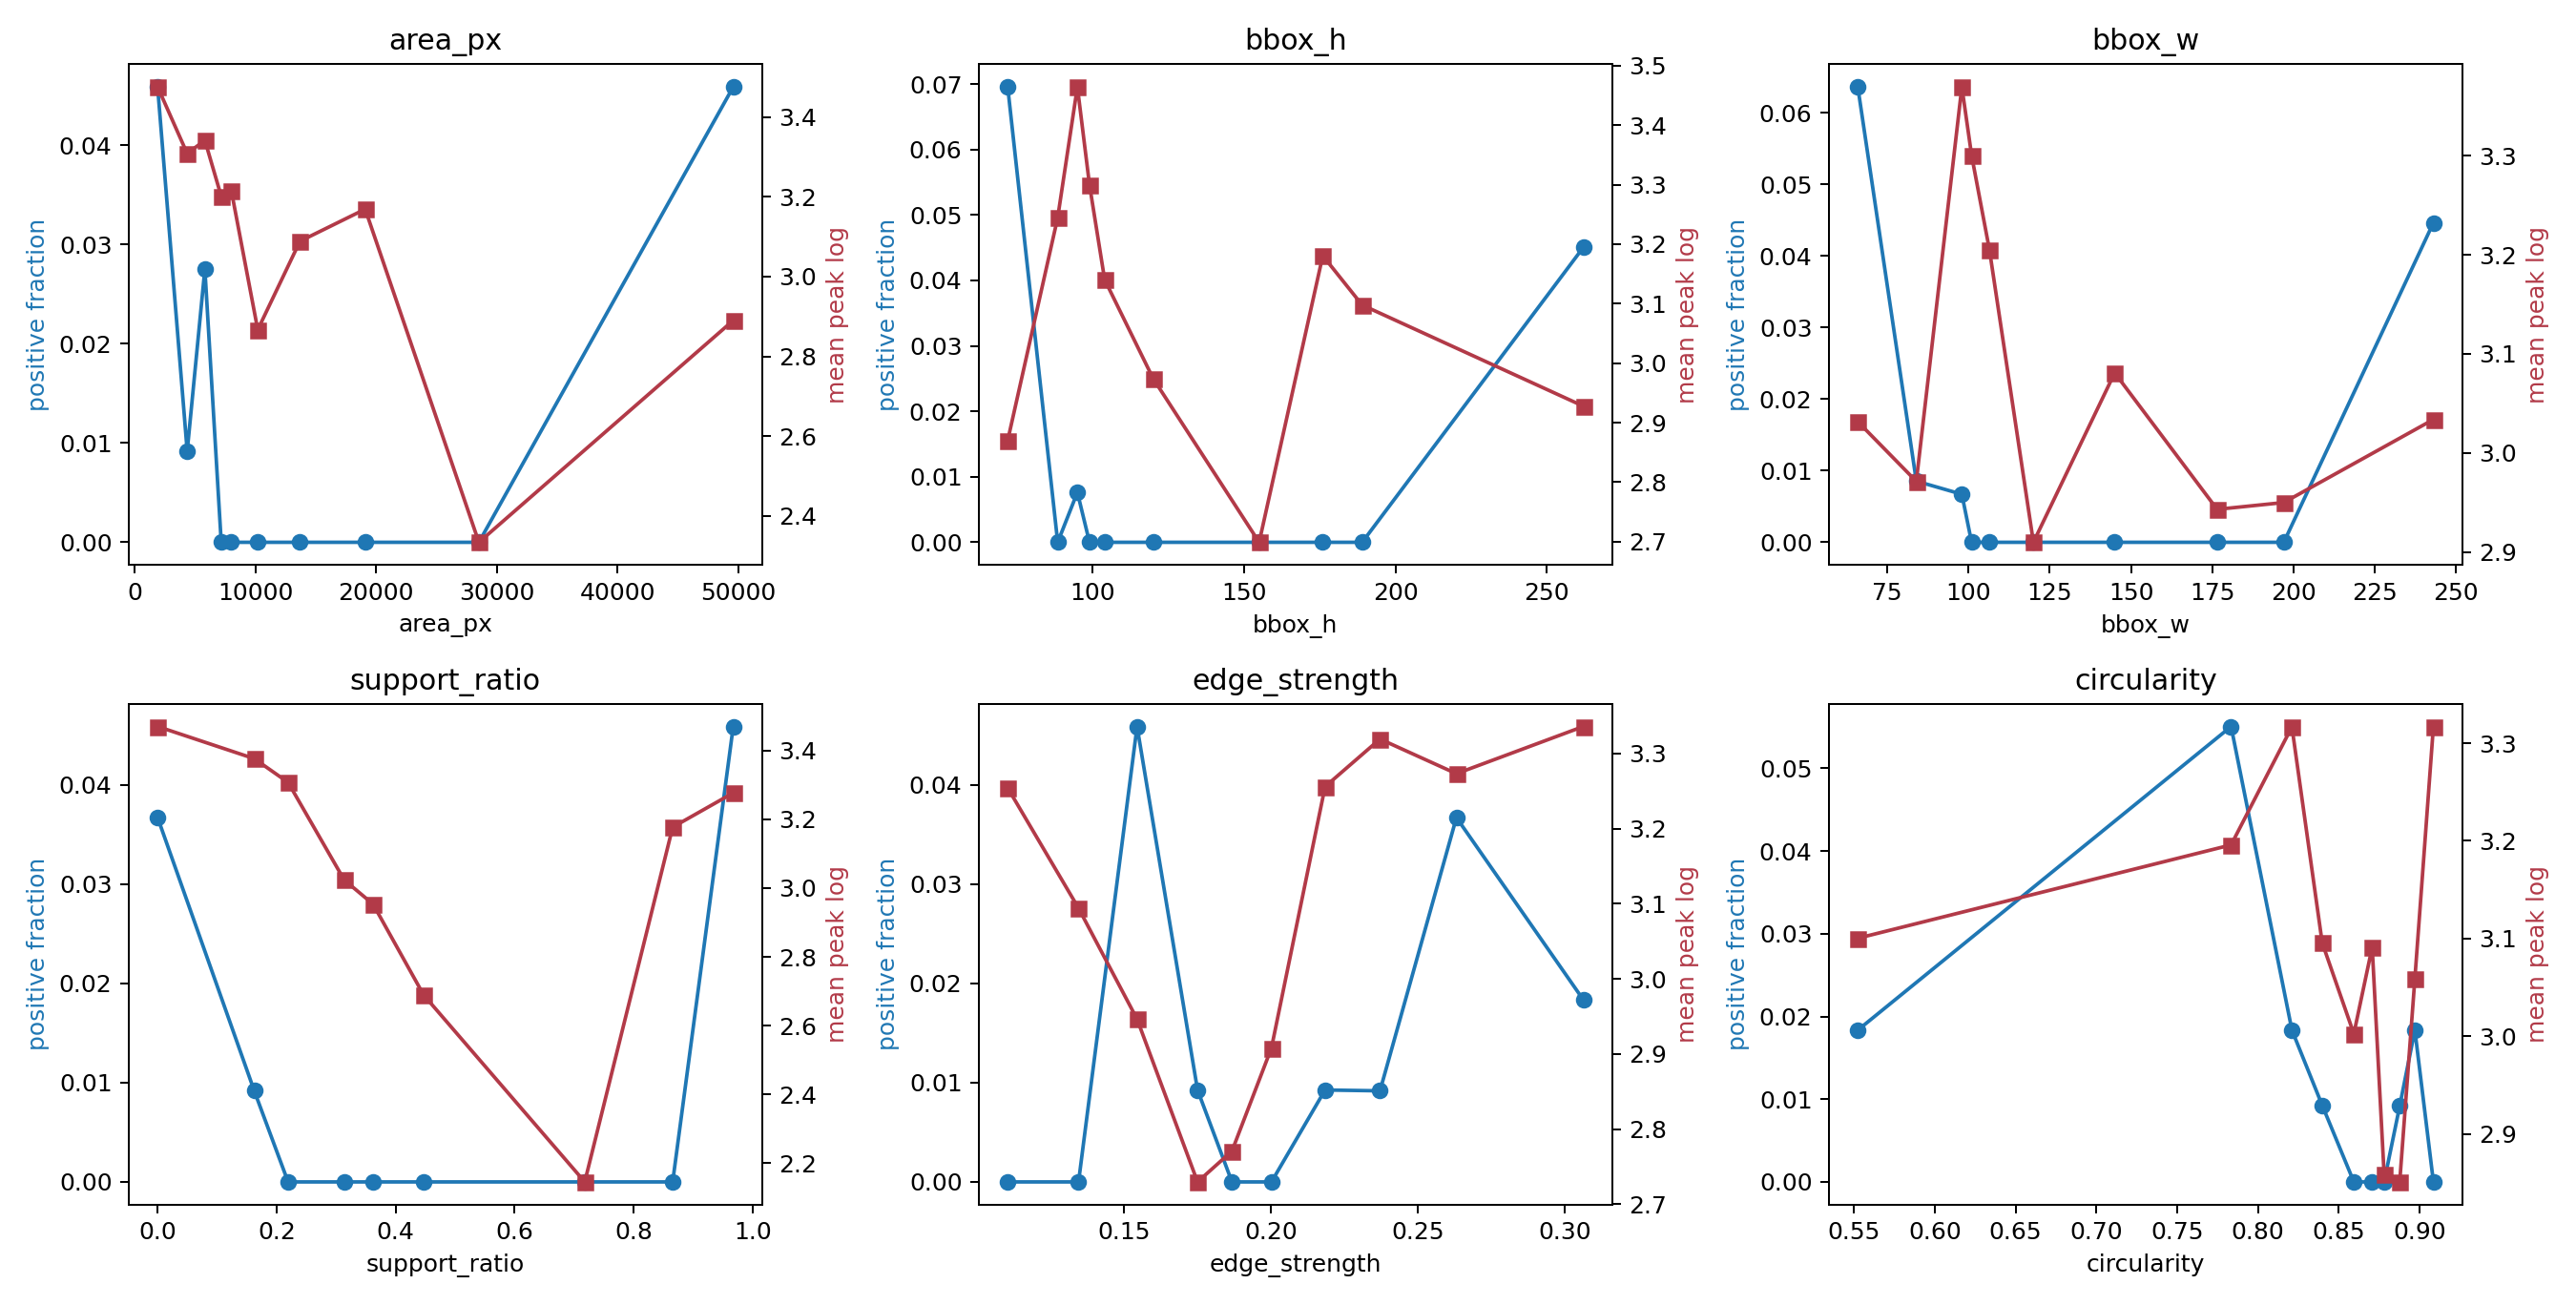
\includegraphics[width=\linewidth]{figures/fig4_b2f_feature_trends.png}
\caption{Feature trend plots from the separate B2F evaluation.}
\label{fig:b2f-feature-trends}
\end{figure}

\section{Separate Model 2: Scalar Future Prediction}

The scalar future model takes a prefix of earlier brightfield crops and explicit features:
\begin{equation}
P_k = \{(B_j, X_j)\}_{j=k-L+1}^{k}, \quad L \leq 5,
\end{equation}
and predicts future-expression status, future peak fluorescence, and future fluorescence AUC:
\begin{equation}
(\hat{y}_p,\hat{r}_p,\hat{q}_p) = H_\phi(P_k), \quad p > k.
\end{equation}

\begin{table}[H]
\centering
\caption{Held-out scalar future metrics from \texttt{stage2\_future\_expression/test\_metrics.json}.}
\begin{tabular}{lc}
\toprule
Metric & Value \\
\midrule
Test prefix samples & 633 \\
Expression AUROC & 0.228 \\
Average precision & 0.0156 \\
Future peak Pearson correlation & 0.134 \\
Future AUC Pearson correlation & 0.105 \\
Future peak MAE & 0.579 \\
Future AUC MAE & 0.929 \\
Image target & Not predicted \\
\bottomrule
\end{tabular}
\end{table}

\begin{figure}[H]
\centering
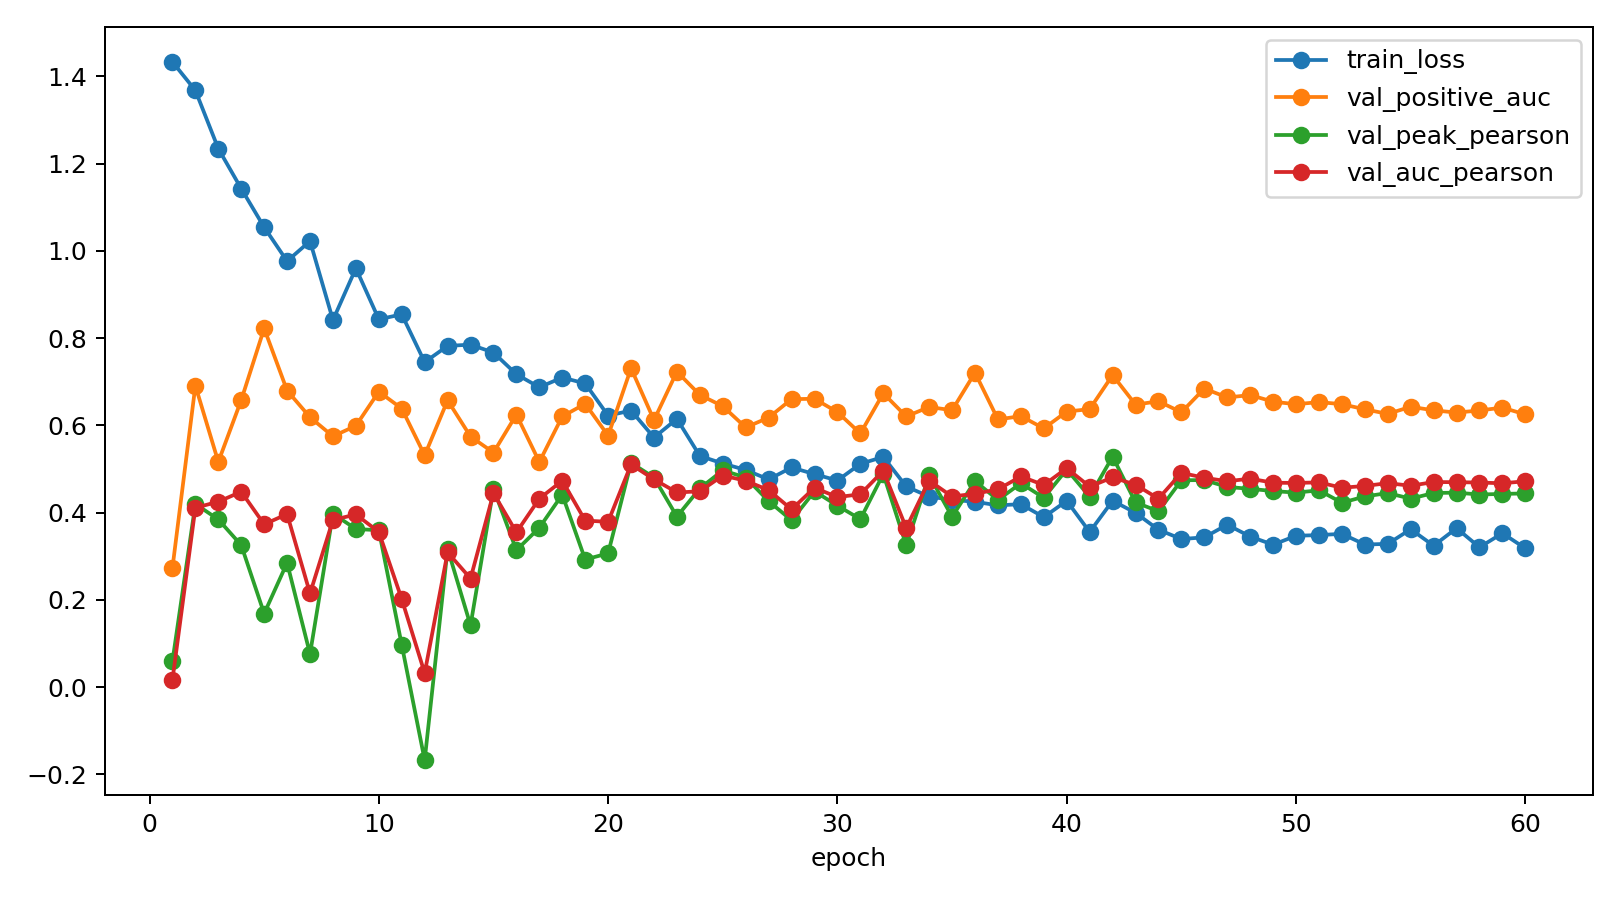
\includegraphics[width=0.9\linewidth]{figures/fig5_scalar_future_training_metrics.png}
\caption{Training curves for the separately trained scalar future model.}
\label{fig:scalar-training}
\end{figure}

\begin{figure}[H]
\centering
\begin{subfigure}[b]{0.49\linewidth}
\centering
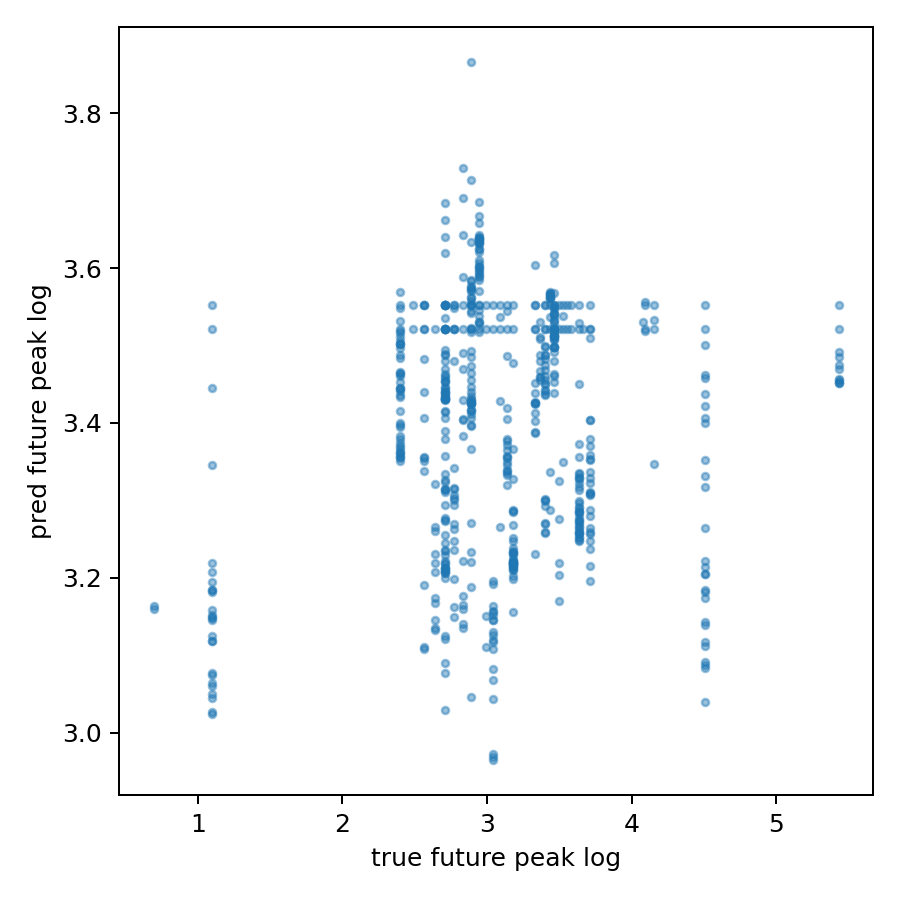
\includegraphics[width=\linewidth]{figures/fig6_scalar_future_peak_scatter.png}
\caption{Future peak prediction}
\end{subfigure}
\hfill
\begin{subfigure}[b]{0.49\linewidth}
\centering
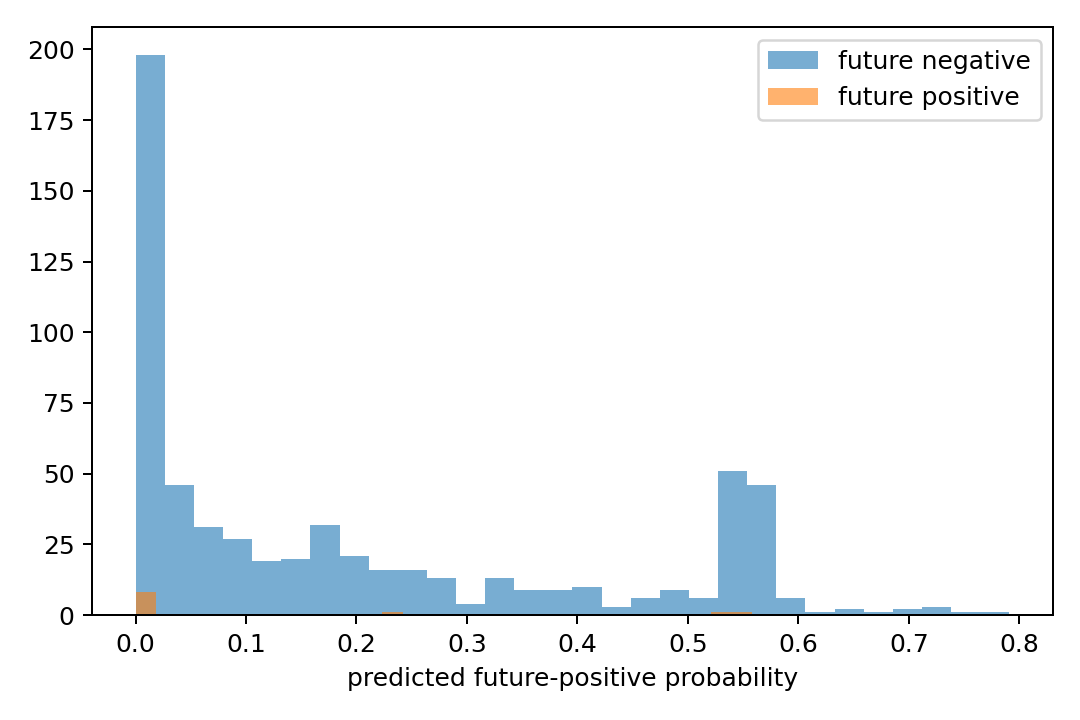
\includegraphics[width=\linewidth]{figures/fig7_scalar_future_score_histogram.png}
\caption{Future-expression score distribution}
\end{subfigure}
\caption{Held-out scalar future outputs. The predicted future scalar values are not close enough to the true future values for useful inference.}
\label{fig:scalar-future}
\end{figure}

\section{Interpretation}

The separate training result is asymmetric. Same-time B2F has measurable signal and should be kept. The separate scalar future model is not sufficient because it discards dense future image structure, relies heavily on approximate track-derived labels, and has too few future-expression examples in the held-out split.

\section{Recommended Use}

\begin{enumerate}
\item Use the B2F model as pretraining for future models rather than treating it as the final biological objective.
\item Do not rely on the separate scalar model alone for future-expression claims.
\item Keep 256$\times$256 as the fast baseline, but test 384$\times$384 or 512$\times$512 because the relevant fluorescent cells can be thin peripheral structures.
\item Improve target construction before scaling model size: verify tracks, use horizon-specific targets, and compare last-future, peak-future, and first-expression-time targets.
\end{enumerate}

\section{Conclusion}

The separate experiments show that brightfield can predict same-time fluorescence better than chance, but the separately trained scalar future model does not yet solve early future-expression prediction. The strongest next step is to reuse the B2F representation inside a joint temporal model, not to treat the separate scalar future model as sufficient.

\end{document}
